%! Author = Vova
%! Date = 13.07.2021

% Preamble
\documentclass[11pt]{article}


% Packages
\usepackage{amsmath}
\usepackage{hyperref}
\usepackage{polyglossia}
\usepackage{graphicx}
\usepackage{babel,blindtext}
\usepackage{subfig}
\usepackage{iftex}

% Language and Font settings

% Kurale
% New Standard Old
\setdefaultlanguage{russian}
\setmainfont[Ligatures=TeX]{Kurale}
\newfontfamily\cyrillicfont{Kurale}

% Author, date
\title{Описание программной части робота-художника}
\author{Латыпов Владимир Витальевич}
\date{\today}

% Graphics settings
\graphicspath{{../images/}}

% Document
\begin{document}
    \maketitle
    \newpage
    \tableofcontents
    \newpage

    \section{Формулировка задачи}

    Для того, чтобы робот-художник нарисовал что-либо, ему нужно предоставить данные в определённом формате, а именно — не набор пикселей,
    как требуется для показа на мониторе, а набор «мазков»: это связано с конструкцией самого робота.
    Мазки решено было представлять в виде кривых безье второго порядка (то есть квадратичных), к которым добавлены параметры «толщина» и «цвет».

    Но на вход подаются рисунки не в векторном, а в растровом формате.
    Найти такую комбинацию мазков, которая бы лучше всего соответствовала картине/изображению — задача нетривиальная, имеющая множество решений.

    Конечно же, я выбрал решать задачу самостоятельно, а не использовать готовые библиотеки.

    \section{Описание программы в общих чертах}\label{sec:approx_description}
    Таким образом, решено было использовать эвристические алгоритмы оптимизации:
    \href{https://en.wikipedia.org/wiki/Simulated_annealing}{Генетический алгоритм} и \href{https://en.wikipedia.org/wiki/Simulated_annealing}{Симуляция отжига}.

    \subsection{Задание функции ошибки}
    Функцию ошибки необходимо задать таким образом, чтобы она отражала качество полученной комбинации мазков,
    причём в любой точке направление её уменьшения соответствовало направлению улучшения результата.
    Помимо напрашивающегося \href{https://en.wikipedia.org/wiki/Mean_squared_error}{MSE}

    \begin{equation}\label{eq:equation}
        MSE = \sum_{y = 0}^{y < height} { \sum_{x = 0}^{x < width} { \sum_{c \in  \left\{ r, g, b \right\} } { \left( {\overrightarrow {rendered_{x, y}}}_c - {\overrightarrow{original_{x, y}}}_c\right)^2 }}}
    \end{equation}

    , повсеместно используемого при работе с изображениями, функция ошибки «наказывает» наложение мазков, а также

    \subsection{Растеризация мазков}\label{subsec:rasterization}
    Имея мазок, заданный в виде трёх точек на плоскости, толщины и цвета, нужно уметь его отобразить его на «холсте», то есть в виде набора пикселей.
    Это нужно, чтобы подсчитать функцию ошибки для заданного набора мазков.
    Есть много способов произвести растеризацию.

    Самый простой — для некоторого количества точек на кривой Безье (с достаточно маленьким шагом, примерно один пиксель) проводим вертикальную линию: вверх на width и  вниз — тоже.
    Это даёт высокую производительность и сносно выглядит на участках, близких к горизонтальным, но результат, полученный таким способом, очень далёк от реальности на вертикальных участках:
    \begin{figure}[h!]
        \centering
        \includegraphics[width=0.75\textwidth]{stroke_vertical.png}
        \caption{(Красным обозначены точки, задающие кривую)}
        \label{fig:vertical_stroke}
    \end{figure}
    \begin{figure}
        \centering
        \includegraphics[width=0.75\textwidth]{one_stroke.png}
        \caption{Иногда такой способ добавляет свой шарм}
        \label{fig:pretty_vert_stroke}
    \end{figure}

    Есть разные способы избавиться от этих недостатков, сохраняя максимальную производительность.
    Например:
    \begin{itemize}
        \item Совмещать горизонтальные и вертикаьлные полосы
        \item Проводить полосы перпендикулярно направлению кривой в данной точке
    \end{itemize}
    В каждом из них будут наблюдаться пустые места, полости, что недопустимо.

    Ультимативным же способом является подражание реальной жизни: «проведение» круглой «кистью» по экрану.
    То есть берутся точки на кривой на небольшом расстоянии друг от друга, и с центром в каждой из них рисуется круг радиусом width.
    Однако в таком случае каждая точка, попадающая в мазок обрабатывается много раз (для близких кругов), что значительно замедляет рендерниг.
    Если же увеличить шаг, этой проблемы можно частично избежать, но мазок стал бы неровным.
    При маленьком шаге это выглядит так:
    \begin{figure}[h!]
        \centering
        \includegraphics[width=0.75\textwidth]{stroke_smooth.png}
        \label{fig:smooth_stroke}
    \end{figure}

    В будущем планируется улучшить алгоритм для ускорения растеризации при почти том же качестве.
    Рассматриваются варианты:
    \begin{itemize}
        \item Заменить круглую кисть на также гладкую, но с более медленным закруглением с дальней от вектора кривой в данной точке стороны, поворачивая кисть соответствующим образом:
        \begin{figure}
            \centering
            \includegraphics{modern_brush.png}
            \caption{(красным обозначено направление вектора кривой)}
            \label{fig:modern_brush}
        \end{figure}
        Такое изменение поможет уменьшить артефакты при увеличении шага между точками на кривой, то есть позволит сделать шаг больше, ускорив процесс.

        \item Автоматически разбивать мазок на «полигоны».
                    Для этого нужно пройтись по кривой и с некоторым шагом (уже побольше, чем раньше),
                    отметить для каждой рассматриваемой точки на прямой, содержащей её и перпендикулярной текущему направлению, точки в обе стороны от неё на расстоянии width.
                    Каждая из них добавляется в соответствующий стороне в порядке обхода список.
                    Потом полигоны, полученные из соседних точек на кривой и соответствующим им вынесенным точкам, заливаются нужным цветом.
                    На концах же мазка рендерятся круги.

        \begin{figure}
            \centering
            \includegraphics{polygonal_stroke.png}
            \caption{Схема полигональной разбивки мазка}
            \label{fig:polygonal_stroke}
        \end{figure}

    \end{itemize}

    \section{Технические аспекты}\label{sec:tecnical}

    \subsection{Основное}\label{subsec:major}
    Программа написана на языке программирования C++(так как требовалась максимальная скорость), сборка осуществляется с помощью CMake.
    Проект можно скомпилировать под Windows (компилятор MSVC) и под Linux (тестировалось на g++-10).

    Код хранится в \href{https://github.com/donRumata03/Painter}{guthub-репозитории (кликабельно)}.

    \subsection{Библиотеки}\label{subsec:libs}

    \subsubsection{OpenCV}
    Для работы с изображениями используется OpenCV, но не модуль машинного обучения, а лишь примитивные операции с изображениями:
    прочтение из популярных форматов, сохранение в них, хранение и копирование матрицы пикселей и т.д.

    \subsubsection{Pythonic}
    Для работы проекта также необходима библиотека «\href{https://github.com/donRumata03/pythonic}{pythonic}»: она написана мной, подключается также через CMake.
    Она отвечает за базовые функции и структуры данных.
    Я использую её во всех более или менее крупных проектах на C++.
    В ней на данный момент есть:
    \begin{itemize}
        \item Простые вспомогательные функции для работы со строками, контейнерами, форматированного вывода
        \item Вызов питоновской библиотеки matplotlib для построения графиков
        \item Базовые алгоритмы наподобие бинарного поиска и дерева отрезков
        \item Функционал для работы со временем, в том числе — анализатор последовательных запусков процесса
        \item Платформонезависимая работа с кодировками и файловыми системами
        \item Примитивы для вычислительной геометрии
        \item Функции для работы со статистикой
        \item Многомерный шаблонный массив с количеством измерений, изменяемом в run-time
        \item Сглаживание функций и построение примерной функции распределения в пространстве с заданной размерностью по набору sampl-ов с помощью гауссовых ворот
        \item Функционал для работы с многопоточностью, в том числе — thread pool, умеющий снимать нагрузку с ожидающих потоков с помощью std::condition\_variable.
    \end{itemize}

    \subsubsection{lunasvg}
    Для работы с SVG используется библиотека \href{https://github.com/sammycage/lunasvg}{lunasvg}.
    P. S. У этой библиотеки отличный автор, он изучает проекты, в которых библиотека используется, и пишет рекомендации о best prictice её использования.

    \subsubsection{PowerfulGA}
    Функционал по методам оптимизации реализован мной и вынесен в отдельную репозиторию: \href{https://github.com/donRumata03/PowerfulGA}{click}
    (там не только Генетический алгоритм, как можно было подумать из названия, но и симуляция отжига, градиентный спуск, метод Ньютона;
    многие другие алгоритмы планируются быть добавленными)
    Более подробное описание в секции $\longrightarrow$ \ref{sec:opimization_algorithms}

    \section {Алгоритмы оптимизации}\label{sec:opimization_algorithms}
    \subsection{Общий принцип ГА}\label{subsec:ga_general_principles}
Идея работы генетического алгоритма заимствована у природы: также, как в ходе эволюции, происходит появление оптимального организма для заданных условий — в ходе работы алгоритма ищется набор параметров, при котором фитнесс-функция максимальна.

В природе тот, кто лучше приспособлен к окружающей среде, в большей степени получает доступ к размножению,
в результате чего новые особи получают признаки от лучших родителей.
Из-за того, что геном наследуется от обоих родителей, получившиеся комбинации могут по-новому комбинировать в себе черты,
что даёт большое преимущество перед бесполым размножением (аналогом которого являются такие методы оптимизации, как градиентный спуск или отжиг).
Нужно пояснить, что половое размножение не обязательно предполагает наличие нескольких полов.
Особи в ГА — аналоги гермафродитов из живой природы: в отличие от людей, каждая особь может скрещиваться с каждой.

Это позволяет именно лучшим чертам, по каким-либо причинам появившихся у особей, переходить в следующее поколение.

За их появление отвечают мутации — небольшие случайные изменения в геноме.

Из принципа работы можно понять, что алгоритм \href{https://en.wikipedia.org/wiki/Heuristic_(computer_science)}{эвристический}: сложно доказать его сходимость или что-либо гарантировать с вероятностью 100\%.
Зато исследования (\url{talgat.org/news/wp-content/uploads/2018/08/112.pdf}) показывают, что именно этот алгоритм даёт лучшие результаты для самых сложных функций.
В разделе \ref{subsubsec:hazing}, какие меры предпринимаются, чтобы не дать алгоритму попасть в локальный минимум, не добравшись до глобального.

\subsection{Термины}\label{subsec:ga_principles}
Набор параметров представляется в виде \textit{«генома»} — некой структуры данных, содержащей информацию об этом наборе.
\textit{Особь} — в контексте алгоритма будет использоваться в качестве синонима к геному.

Геном состоит из \textit{генов} — каждый из них содержит информацию о каком-либо признаке (в случае природы) или параметре (в случае ГА).

В каждый момент времени алгоритм работает с \textit{популяцией} — набором геномов.
Это аналог популяции в природе.

Мутация — как и в реальной жизни — небольшое случайное изменение генома без строго определённого направления.

\subsection{Примерная последовательность действий ГА}\label{subsec:approx_ga_algo}
В общих чертах работа ГА выглядит так:

\underline{Инициализация}: Сгенерировать случайную популяцию, каждый ген каждого генома — в заданных пределах.

Затем — повторять, пока не закончится заданное количество итераций или не будет достигнуто требуемое значение фитнесс-функции:

\begin{enumerate}
    \item Посчитать фитнесс-функции для каждой из особей.
    Для большинства задач этот шаг занимает бо́льшую часть времени исполнения,
    поэтому нужно оптимизировать именно его, в частности — распараллелить,
    запуская независимые вычисления на нескольких потоках.

    \item Каким-либо образом отобрать особи на скрещивание

    \item Произвести скрещивание, получив «отпрысков» — часть нового поколения

    \item Сформировать новое поколение, используя, возможно, в разных пропорциях, различные источники геномов, а именно:

    \begin{itemize}

        \item Отпрысков, полученных на предыдущем шаге в результате скрещивания
        \item Лучшие особи из прошлой популяции

        \item Случайные особи — чтобы не дать алгоритму сойтись раньше времени, попав в локальный минимум

        \item Возможно, результаты скрещивания одновременно более двух особей.

    \end{itemize}

    \item Произвести мутации в некоторых особях этого поколения (лучшие из мутаций внедрятся в популяцию на следующих итерациях).

    \item Опционально — «обрезать» (то есть насильственно подправить)
    те мутации, которые привели к выходу каких-либо параметров или их комбинаций за пределы допустимого.

    \item Если алгоритм подходит к концу, добавить лучший геном из предыдущего поколения (чтобы он не подвергся мутации)

\end{enumerate}

\subsection{Конкретная реализация ГА и авторские модификации}\label{subsec:my_modifications}

Учитывая тот факт, что в большинстве задач, решаемых мною, бо́льшая часть вычислительного времени ($\gg 95\%$) используется для подсчёта функции ошибки, а не для маниппуляций с геномами
(это подтверждается результатами профайлинга),
задача состоит в том, чтобы минимизировать количество подсчётов функции ошибки, пусть и ценой более долгой работы с геномами.

Первое изменение — отказ от дискретного кодирования геномов.

Для алгоритма по каждой переменной задан её диапазон.

Традиционный подход — разделить диапазон на $2^N$ частей и кодировать номер части в геноме как битовую последовательность из $N$ бит.
Для подсчёта функции ошибки этот номер перекодируется назад в соответствующую точку непрерывной величины.
Мутацией в данном случае является изменение случайного количества каких-то битов этого номера.

А скрещивание обычно происходит путём случайного выбора значений каждого из двоичных разрядов в родительских геномах.

Предварительное тестирование показало бо́льшую эффективность хранения самого числа (без кодирования) по сравнению с традиционным подходом (хранение битовой последовательности), однако планируется провести более тщательное тестирование (см. \ref{itm:testing_system})

\subsection{Операция «скрещивание»}\label{subsec:matting}

Выбор особей для скрещивания происходит пропорционально значению фитнесс-функции в некоторой (небольшой) степени,
что увеличивает разнообразие, так как в случае небольшой степени «оригинальные» геномы, но с неидеальной функцией ошибки могут попасть в «отцы».

Для реализации используется «рулетка» с кумулятивными вероятностями и бинарный поиск по ней при генерации новой особи по случайному числу от 0 до 1.

Само размножение (по умолчанию) осуществляется так: имея два родителя, каждый ген с некоторой вероятностью
либо берётся от отца, либо от матери, либо (так как это непрерывный вещественный параметр)
генерируется по такой плотности вероятности (значения параметра у двух родителей — два крайних максимума на этой кривой):

\begin{figure}[h!]
    \centering
    \includegraphics[width=0.75\textwidth]{matting.jpeg}
    \caption{Синяя кривая — для близких геномов, оранжевая — для более далёких}
    \label{fig:}
\end{figure}
\FloatBarrier

Кривая формируется через сумму трёх нормальных распределений.

Она было подобрано таким образом, чтобы наилучшим образом раскрывались
потенциальные возможности генетического материала: максимумы, например, наблюдаются в изначальных точках
и в центре между ними — это именно то, что может нам «дать» такой генетический материал.

Факт в том, что при использовании обычного бинарного кодирования просто-напросто
дискредитируется изначальная природа данных, что не позволяет достичь хороших результатов.

\subsubsection{hazing\_percent: скорость сходимости}\label{subsubsec:hazing}

При использовании алгоритма оптимизации должен поддерживаться баланс
между скоростью сходимости и избежанием застревания в локальном оптимуме.

В случае моей модификации ГА этот баланс регулируется коэффициентом hazing\_percent.

При формировании новой популяции, как было сказано выше, используются разные категории геномов:

\begin{itemize}

    \item Некоторое количество отпрыски, полученные на предыдущем шаге в результате скрещивания (Подробнее про это — в разделе~\ref{subsec:matting}): назовём их $children$.
    \item Иногда — лучшая особь из предыдущей популяции (одна) — $best\_genome$.
    \item Некий набор «элитарных» геномов ($elite$) — отбор на эти места осущевляется пропорционально фитнесс-функции также в некой степени, но уже в большей,
            что делается её действительно элитной.

    \item Гиперэлита ($hyper\_elite$) — то же самое, но меньше мест и больше степень.

    \item … (Остальные)

\end{itemize}

Изменяя распределения мест по категориям, можно регулировать скорость сходимости.
На это распределение и влияет параметр hazing («дедовщина»):
высокое его значение приводит к доминированию уже сформировавшихся геномов и скорейшей их «дошлифовке»,
однако не даёт новым, «подающим надежды» развиться и закрепиться.

Кроме того, в каждой эпохе (итерации) определяется распределение, учитывая процент выполнения алгоритма
— к концу запускается режим максимальной дедовщины: все, кто смог подать надежду, уже закрепились, осталось как раз их «дошлифовать».

(Нужно исследовать всю область поиска,
поэтому нужно не давать сразу огромный бонус при размножении и переходе в другое поколение за некоторое преимущество.)

Только так получится обеспечить развитие нескольких «очагов», внутри которых и будет происходить «шлифование» «идеи искать в этой области».

В будущем планируется сделать распределение мест по степеням отбора непрерывным,
исследовать его, найти оптимальное (возможно — тоже с помощью метаалгоритма оптимизации).



    \section{Наблюдения}\label{sec:observations}

    \subsection{Неравенство зон}\label{subsec:inequality}
    Когда я заметил, что зоны, на которые Adobe Illustrator делит изображение, могут очень сильно отличаться в размере (отношение площадей может достигать 1000 раз),
    мне захотелось измерить это неравенство численно, чтобы при разработке нового алгоритма измерять его качество в том числе по этому параметру.

    Существует большое количество метрик, я решил выбрать основные из них:
    \begin{itemize}
        \item Индекс Джини (вместе с кумулятивным графиком распределения дохода (также известен как \href{https://en.wikipedia.org/wiki/Lorenz_curve}{кривая Лоренца}))
        \item Процент «дохода» 1\% самых богатых от общего «дохода» (В случае зон вместо дохода используется занимаемая площадь).
        \item Процент самых богатых, имеющих в сумме 50\% от общего дохода.
    \end{itemize}

    Индекс Джини рассчитывается как отношение площади между кривой Лоренца и «линией равенства» к площади под линией равенства.
    Иными словами, $G = \frac{A}{A + B}$ на этой схеме:

    \begin{figure}[h!]\label{fig:lorenz_curve}
        \centering
        \includegraphics[width=0.75\textwidth]{typical_lorenz_curve.png}
        \caption{Типичная кривая Лоренца}
    \end{figure}
    Альтернативный способ посчитать коэффициент, использующийся в реализации:
    \begin{equation}
        G = \frac{\sum_{i=1}^{n}  \sum_{j=i+1}^{n}  \left| y_i - y_j \right|}{n \cdot \sum_{i=1}^{n} y_i}
    \end{equation}
    Чем индекс выше, тем большее неравенство наблюдается в стране.
    Более того, использование именно этой метрики позволяет комплексно оценить неравенство между анализируемыми объектами —
    в отличие от рассмотрения процентов дохода заданного квантиля.


    Результаты оказались впечатляющими:
    \begin{itemize}
        \item $Gini\_index \approx 76\%$
        \item 1\% крупнейших зон покрывают ≈ 18\% изображения
        \item 6.25\% зон покрывают половину изображения
    \end{itemize}

    Так выглядит кумулятивный график распределения площади:
    \begin{figure}[h!]\label{fig:cumulative_inequality_graph}
        \centering
        \includegraphics[width=0.75\textwidth]{cumulative_inequality_graph.jpg}
        \caption{Кривая лоренца для зон}
    \end{figure}

    Нетрудно заметить, что ни в одной стране мира нет такого неравенства, как среди зон:

    \begin{figure}[h!]\label{fig:gini_index_world}
        \centering
        \includegraphics[width=0.75\textwidth]{gini_index_world.jpg}
        \caption{Индекс Джини по странам мира}
    \end{figure}
    Даже в ЮАР индекс Джини составляет 57.8\%.


    \section{Дальнейшее развитие}\label{sec:todo}
    Несмотря на то, что программа уже работоспособна, есть ещё много идей и планов по её усовершенствованию:
    \begin{itemize}
        \item Внедрить \textit{быстрый пересчёт функции ошибки} — это улучшение давно напрашивается,
                но оно несколько теряет в эффективности из-за того, что в одной мутации в среднем изменяется
                не так мало мазков (однако это количество убывает со временем).
                В настоящий момент ведётся работа над внедрением.
        \item Разделение мазков по слоям.
                Нетрудно заметить, что при рисовании картин художники сначала проходятся по холсту черновыми мазками большого размера, а затем — прорабатывают детали.
                Таких уровней детализации зачастую бывает немало.

        Пример того, как художник (\href{https://www.youtube.com/watch?v=VaXHtai2alU}{https://www.youtube.com/watch?v=VaXHtai2alU}) рисует картину по слоям:


        \begin{figure}[h!]
            \centering
            \subfloat{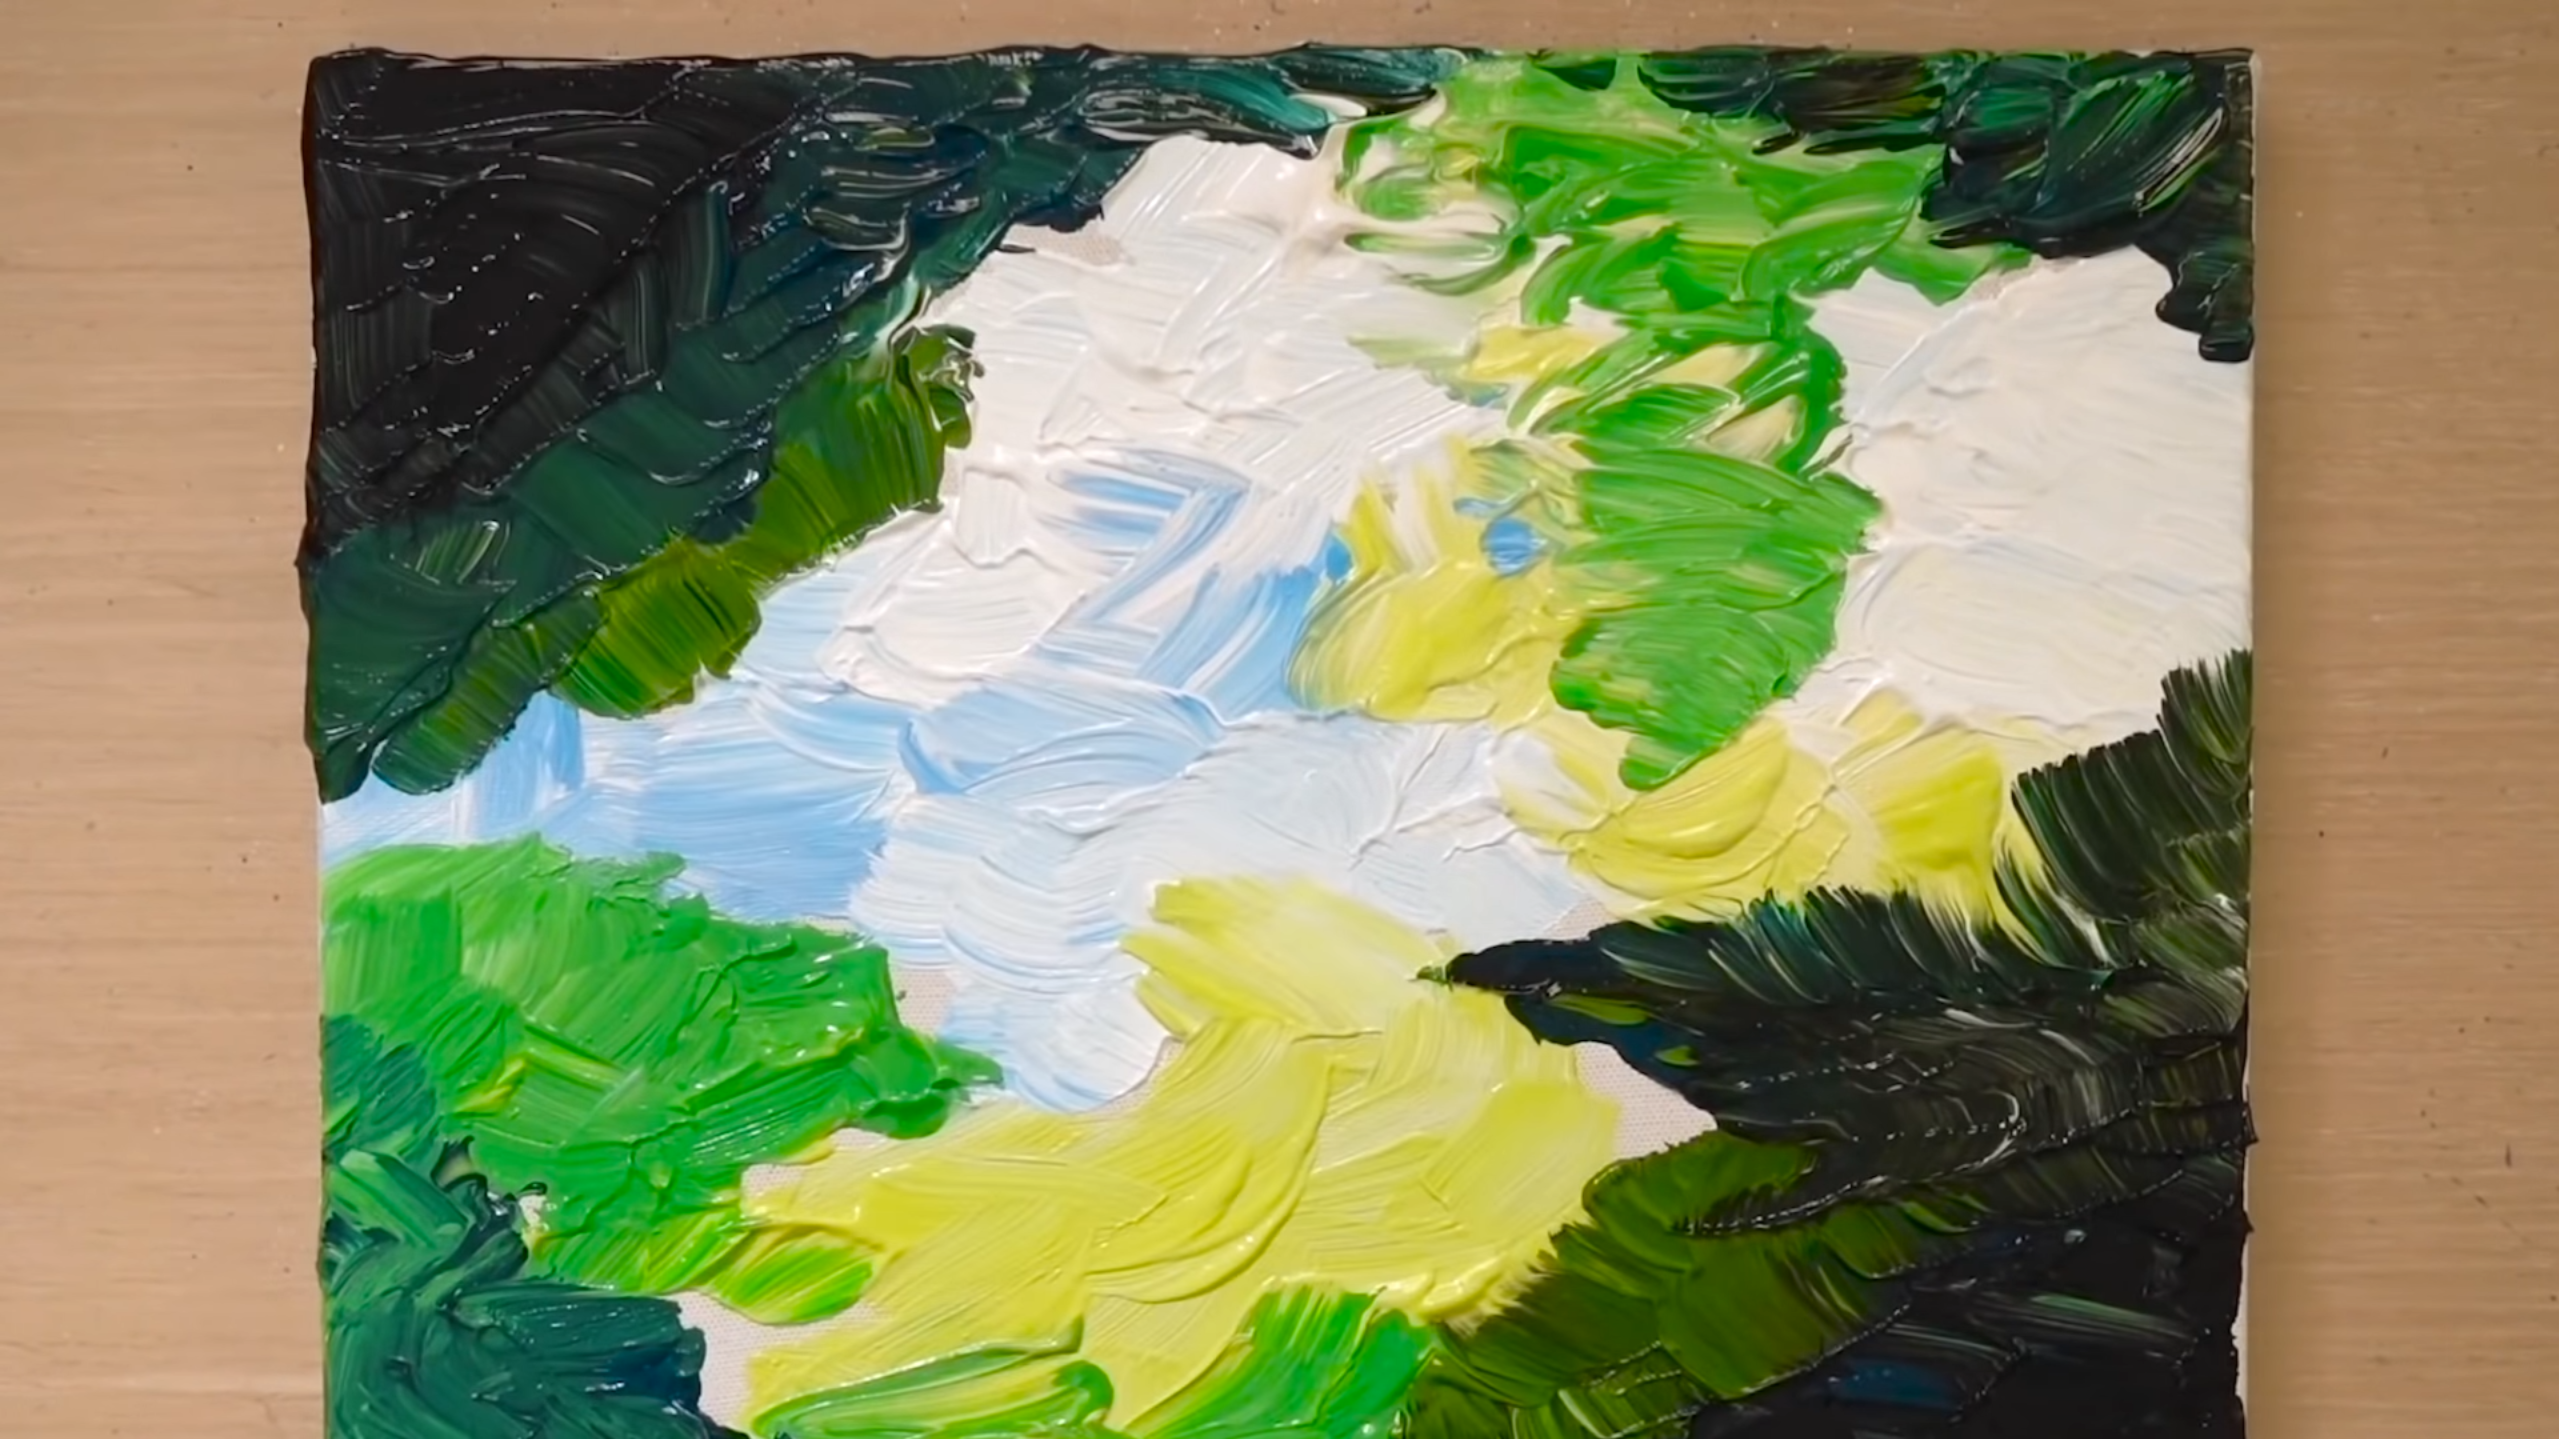
\includegraphics[width=0.24\textwidth]{painting_example_layer_0.png}}
            \subfloat{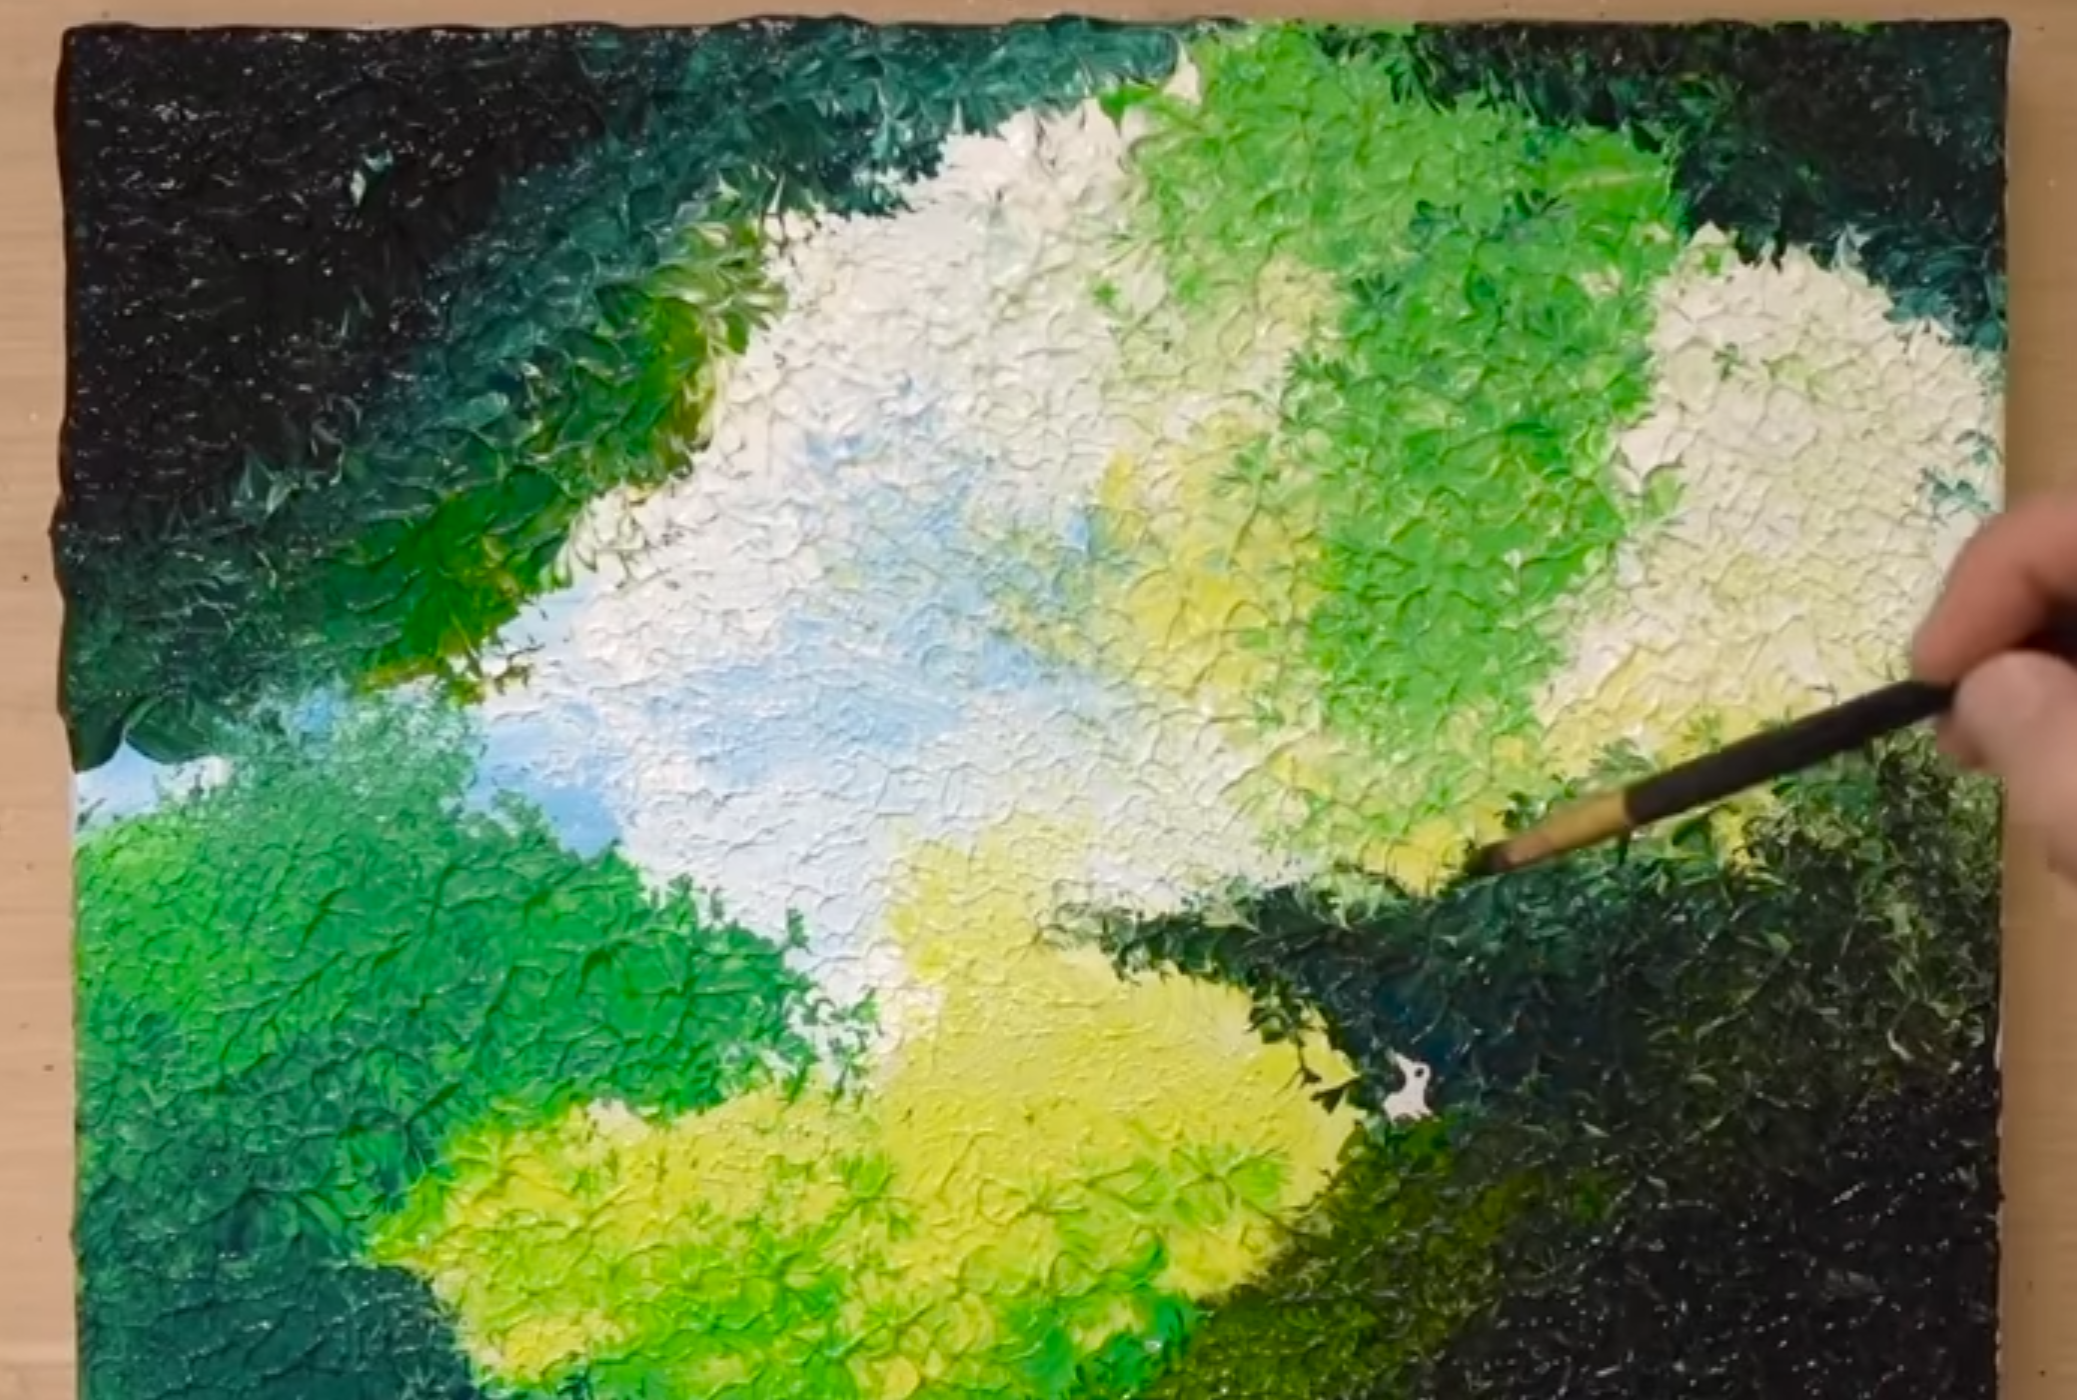
\includegraphics[width=0.24\textwidth]{painting_example_layer_1.png}}
            \subfloat{\includegraphics[width=0.24\textwidth]{painting_example_layer_2.png}}
            \subfloat{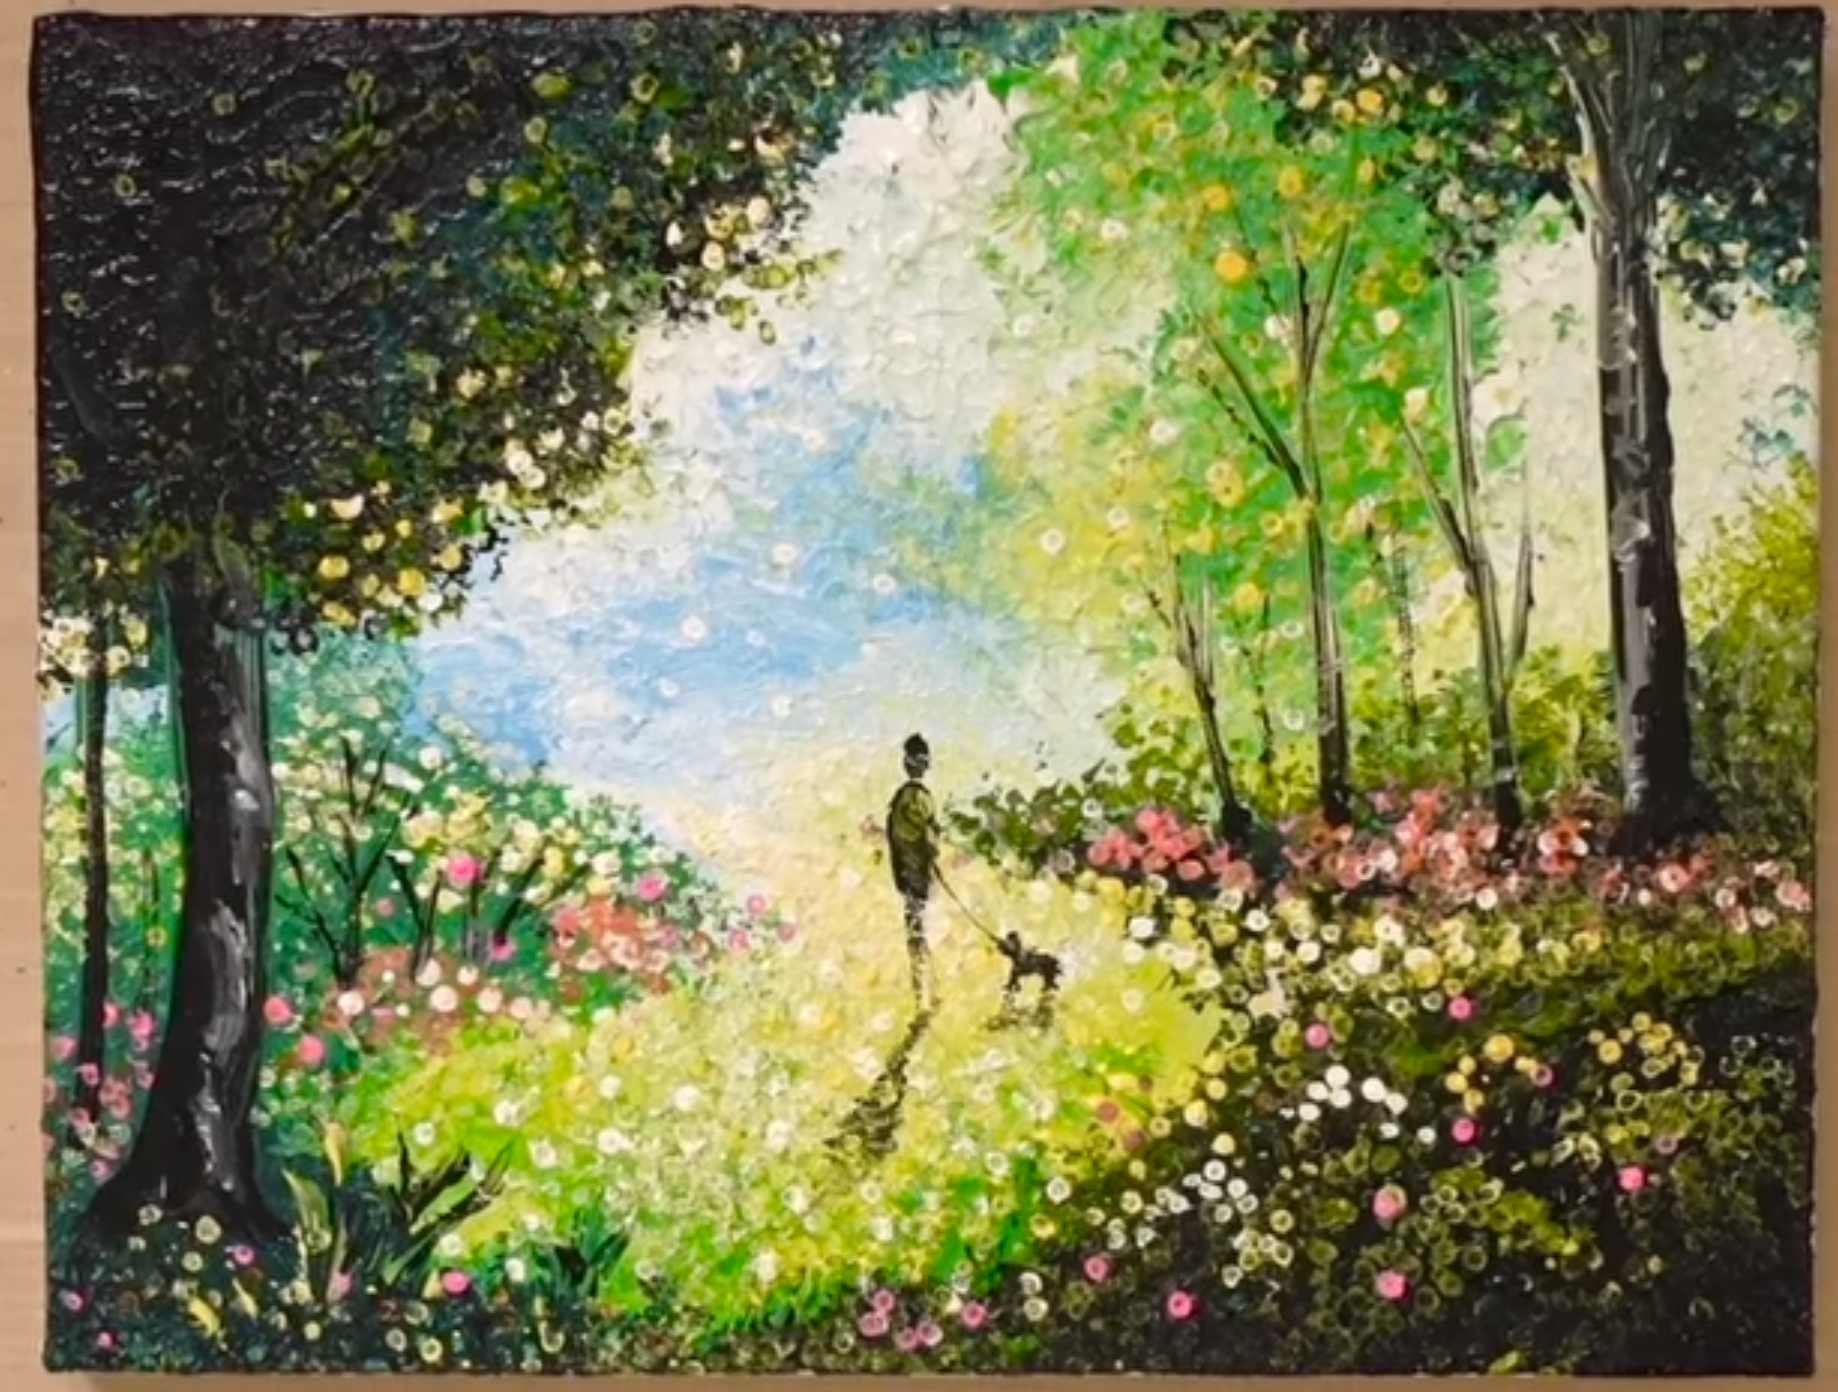
\includegraphics[width=0.24\textwidth]{painting_example_layer_3.png}}
            \caption{ Фон | Рельеф фона | Детализация заднего плана | Основные объекты}
            \label{fig:layered_painting}
        \end{figure}


                Поэтому стоит попробовать сначала заполнять картинку толстыми, грубыми мазками
                (то есть просто с большей шириной, а в реальной жизни это будет отражаться в большем размере кисти и в более сильном нажатии).
        \item Добавить использование локальных методов оптимизации.
                Такие методы, как \textbf\textit{{градиентный спуск}} и \textbf\textit{{метод Ньютона}} позволяют достичь гораздо большей скорости сходимости
                (в случае метода ньютона — сходимость \href{http://w.ict.nsc.ru/books/textbooks/akhmerov/mo_unicode/4.html}{квадратичная}),
                но требуют умения посчитать градиент функции ошибки в любой точке, а также вектор вторых производных по каждому из аргументов.

                Сами алгоритмы реализованы и находятся в \href{https://github.com/donRumata03/PowerfulGA/blob/master/other_optimization/local_optimization.cpp}{этой папке}.
                Предусмотрена опция подсчёта первой и вторых производных через подстановку близких значений параметров:

                \begin{equation}
                    f'(x_0) \approx \frac{f(x_0 + \Delta x) - f(x_0)}{\Delta x}
                \end{equation}

                Однако в случае с мазками при маленьких изменениях параметров функция ошибки остаётся неизменной, так как это приводит к такому же набору закрашенных пикселей.
                Соответственно, нужно либо радикально увеличивать разрешение изображения, либо использовать аналитические методы.
                То есть нужно математически посчитать изменение функции ошибки при бесконечно малом изменении из параметров функции.

        \item \label{itm:testing_system} Организовать систему тестирования различных алгоритмов на различных функциях.
        Звучит как нечто весьма простое, но реальность сложнее, чем кажется.
        Напрашивающийся вариант — дать каждому алгоритму заданное количество вычислений функции ошибки и сравнить, какой результат они получат.

        Однако функция ошибки нелинейная, поэтому сложно будет понять,
        насколько сильному различию в качестве алгоритма соответствует полученная численная разница в результатах.

        Целесообразно сравнивать количество итераций, требующееся алгоритмам для получения заданного результата.
        Но и тут не всё так просто: нельзя просто запустить алгоритмы на неограниченное количество итераций
        и ждать дотижения нужного значения функции,
        так как во многих из них (как минимум — в моей модификации ГА) то,
        как будет проведена каждая отдельная итерация, сильно зависит от процента выполнения на момент её прохождения:
        происходит планирование,  использующее информацию о максимальном количестве итераций.


        Поэтому нет никакого другого выхода, кроме того, чтобы запускать этот алгоритм с рахым количеством итераций и смотреть, когда он в среднем будет доходить до заданного порога.
        Это необходимо автоматизировать.
        В идеальном случае для поиска порога можно было бы использовать бинарный поиск, но в реальности (с поправкой на шум) имеет смысл использовать эвристическую модификацию н-арного поиска (объяснить!).
        Для полной оценки планируется построить график достаточного количества итераций от nребуемого значения функции в интересующей нас зоне.

        \item Улучшить алгоритм поиска цветов и разделения на зоны.

                Сейчас для разделения изображения на зоны используется Adobe Illustrator.
                По заданному количеству цветов (и, следовательно, уровню детализации) он разделяет изображение на зоны,
                присваивая каждой какой-то из цветов палитры так, чтобы он хорошо .
                Сама палитра тоже формируется в ходе работы алгоритма.

                Скорее всего, для этого используется один из популярных алгоритмов, описанных \href{https://en.wikipedia.org/wiki/Color_quantization}{здесь}, или некая проприетарная их вариация.
                Зоны, на которые происходит деление, описываются частями плоскости, ограниченными кривыми безье — «path»  формате $svg$.
                Несмотря на то что формально алгоритм выполняет свою работу, большое количество зон имеет очень продолговатую форму,
                а также наблюдается неимоверный разброс в размерах между разными зонами (см. \ref{subsec:inequality}):
                всё это уменьшает эффективность процесса.


        \item Перенести графические вычисления на видеокарту.
                Также напрашивающееся улучшение.
                Это может существенно ускорить работу алгоритма, но только генетического (так как при отжиге нельзя распараллелить вычисление для целой популяции),
                причём только в случае, если не используется быстрый пересчёт функции ошибки или мутирует очень много мазков одновременно.
                Как бы то ни было, когда-нибудь стоит добавить эту возможность.
                Тестовый проект с использованием OpenCV я уже написал.
                Адаптацию алгоритма под видеокарту можно посмотреть здесь: \ref{subsec:rasterization}.



    \end{itemize}

\end{document}